% !TEX option = -shell-escape
%%%%%%%%%%%%%%%%%%%%%%%%%%%%%%%%%%%%%%%%%%%%%%%%%%%%%%%%%%%%%%%%%%%%%%%
% This work is licensed under the Creative Commons Attribution 4.0
% International License. To view a copy of this license, visit
% http://creativecommons.org/licenses/by/4.0/.
%%%%%%%%%%%%%%%%%%%%%%%%%%%%%%%%%%%%%%%%%%%%%%%%%%%%%%%%%%%%%%%%%%%%%%%
\documentclass[12pt]{../ussci}

\usepackage{siunitx}
\usepackage{graphicx}
\usepackage{mathtools}
\usepackage{microtype}
\usepackage[capitalize]{cleveref}
\usemintedstyle{friendly}
%======================================================================
\addbibresource{NCM-2017.bib}
%======================================================================
\newcommand\papertopic{Reaction Kinetics}
%======================================================================
\DeclareSIUnit\torr{torr}

\title{ UConnRCMPy: Python-based data analysis for Rapid Compression Machines }

\author[1*]{Bryan W.\ Weber}
\author[1]{Chih-Jen Sung}
\affil[1]{Department of Mechanical Engineering, University of Connecticut, Storrs,
CT, USA}
\affil[*]{Corresponding Author: \email{bryan.weber@uconn.edu}}

\begin{document}
\maketitle

%====================================================================
\begin{abstract} % not to exceed 200 words
    The ignition delay of a fuel/air mixture is an important quantity in
    designing combustion devices, and these data are also used to validate
    computational kinetic models for combustion. One of the typical
    experimental devices used to measure the ignition delay is called a
    Rapid Compression Machine (RCM). This paper presents UConnRCMPy, an
    open-source Python package to process experimental data from the RCM at
    the University of Connecticut. Given an experimental measurement,
    UConnRCMPy computes the thermodynamic conditions in the reaction chamber
    of the RCM during an experiment along with the ignition delay.
    UConnRCMPy relies on several packages from the SciPy stack and the
    broader scientific Python community. UConnRCMPy implements an extensible
    framework, so that alternative experimental data formats can be
    incorporated easily. In this way, UConnRCMPy improves the consistency of
    RCM data processing and enables reproducible analysis of the data.
\end{abstract}

% (Provide 2-4 keywords describing your research. Only abbreviations firmly
% established in the field may be used. These keywords will be used for
% sessioning/indexing purposes.)
\begin{keyword}
    chemical kinetics\sep rapid compression machine\sep reproducibility
\end{keyword}

\section{Introduction}\label{introduction}

The world relies heavily on combustion to provide energy in useful and
clean forms for human consumption; in particular, the transportation
sector accounts for nearly \SI{30}{\percent} of the energy use in the United States
and of that, more than \SI{90}{\percent} is supplied by combustion of fossil fuels
\autocite{MER2016}. Unfortunately, emissions from the combustion of
traditional fossil fuels have been implicated in a host of deleterious
effects on human health and the environment \autocite{Avakian2002}. Two
methods are being considered to reduce the impact of fossil fuel
combustion in transportation on the environment, namely: 1) development
of new fuel sources and 2) development of new engine technologies.

The challenge for engineers is that it is not straightforward to combine
new fuels with newly designed engines. Employing computer-aided design
and modeling of new engines with new fuels will be critical to develop
advanced engines to be able to utilize multiple conventional and
alternative fuels. The key to this process is the development of
accurate and predictive combustion models.

One type of data that is particularly relevant to validate models for transportation
applications is the ignition delay. There are several methods to measure the ignition
delay at engine-relevant conditions, including shock tubes and rapid
compression machines (RCMs). The
primary diagnostic in most RCM experiments is the pressure measured as a
function of time in the reaction chamber. This pressure trace is then
processed to extract the ignition delay.

In this paper, the design and operation of a software package to process
the pressure data collected from RCMs is described. Our package, called
UConnRCMPy \autocite{uconnrcmpy}, is designed to analyze the data
acquired from the RCM at the University of Connecticut (UConn). Despite
the initial focus on data from the UConn RCM, the package is designed to
be extensible so that it can be used for data in different formats while
providing a consistent interface to the user.

Recognizing that reproducible research is an important goal for the
scientific community \autocite{NatureEds2016}, and that the code used to
process experimental data is an important part of reproducing research,
the primary goal of UConnRCMPy is to enable consistent, reproducible
analysis of RCM data. Thus, UConnRCMPy offers all of the features
required to process standard RCM data including:

\begin{itemize}
\item
  Filtering and smoothing the raw voltage generated by the pressure
  transducer
\item
  Converting the voltage trace into a pressure trace using settings
  recorded from the RCM
\item
  Processing the pressure trace to determine parameters of interest in
  reporting the experiments, including the ignition delay and
  machine-specific effects on the experiment
\item
  Conducting simulations utilizing the experimental information to
  calculate the temperature during the experiment
\end{itemize}

Previous software used to analyze RCM data has generally been
undocumented and untested code specific to the researcher conducting the
experiments. Moreover, the software typically used to estimate the
temperature in the experiments is difficult to integrate with the data
processing code. To the best of the authors' knowledge, UConnRCMPy is
the first package for analysis of standard RCM data to be presented in
detail in the literature, and it tightly integrates the temperature
estimation routine into the workflow, reducing errors and
inefficiencies.

This paper serves to describe some of the important aspects of RCM data
processing, particularly the choices that the operator must make that
are rarely documented. In addition, as a complement to the in-source
documentation, this paper documents the design choices, interface, and
flexibility of UConnRCMPy.

\section{Background}\label{background}

The RCMs at the University of Connecticut have been described
extensively elsewhere \autocite{Das2012,Mittal2007a}, and
will be summarized here for reference. The RCMs use a single
pneumatically accelerated and hydraulically decelerated piston. In a
typical experiment, the reaction chamber is evacuated to an absolute
pressure near \SI{1}{\torr}, measured by a high-accuracy static pressure
transducer. Next, the reactants are filled in to the desired initial
pressure (\(P_0\)), and a valve on the reaction chamber is closed.
Compression is triggered by a digital control circuit. After
compression, the piston is held in place to create a constant volume
chamber in which reactions proceed. For appropriate combinations of
pressure, temperature, and mixture composition, ignition will occur
after some delay period. A single compression-delay-ignition sequence is
referred to as an experiment or a run. Each experiment is repeated
approximately 5 times at the same nominal initial conditions to ensure
repeatability of the data, and this set of experiments is referred to in
the following as a condition.

The primary diagnostic on the RCM is the reaction chamber pressure,
measured by a dynamic pressure transducer (separate from the static
transducer used to measure \(P_0\)). The pressure trace is processed to
determine the quantities of interest, including the pressure and
temperature at the EOC, \(P_C\) and \(T_C\) respectively, and the
ignition delay, \(\tau\). The ignition delay is typically measured at
several values of \(T_C\) for a given value of \(P_C\) and mixture
composition; this is referred to in the following as a data set.

\section{RCM Signal Processing Procedure}\label{rcm-signal-processing-procedure}

\subsection{Signal measurement}\label{signal-measurement}

The dynamic pressure transducer outputs a charge signal that is
converted to a voltage signal by a charge amplifier with a nominal
output of \SI{0}{\V} prior to the start of compression. In addition, the output
range of \SIrange{0}{10}{\V} is set by the operator to correspond to a
particular pressure range by setting a ``scale factor''. Typical values
for the scale factor range between \SIrange{10}{100}{\bar\per\V}.

The voltage output from the charge amplifier is digitized by a hardware
data acquisition system (DAQ) and recorded into a plain text file by a
LabView Virtual Instrument. The voltage is sampled at a rate chosen by
the operator, typically between \SIrange{50}{100}{\kHz}. This provides
sufficient resolution for events on the order of milliseconds; the
typical ignition delay measured with this RCM approximately ranges from
\SIrange{5}{100}{\ms}.

\begin{figure}[htbp]
\centering
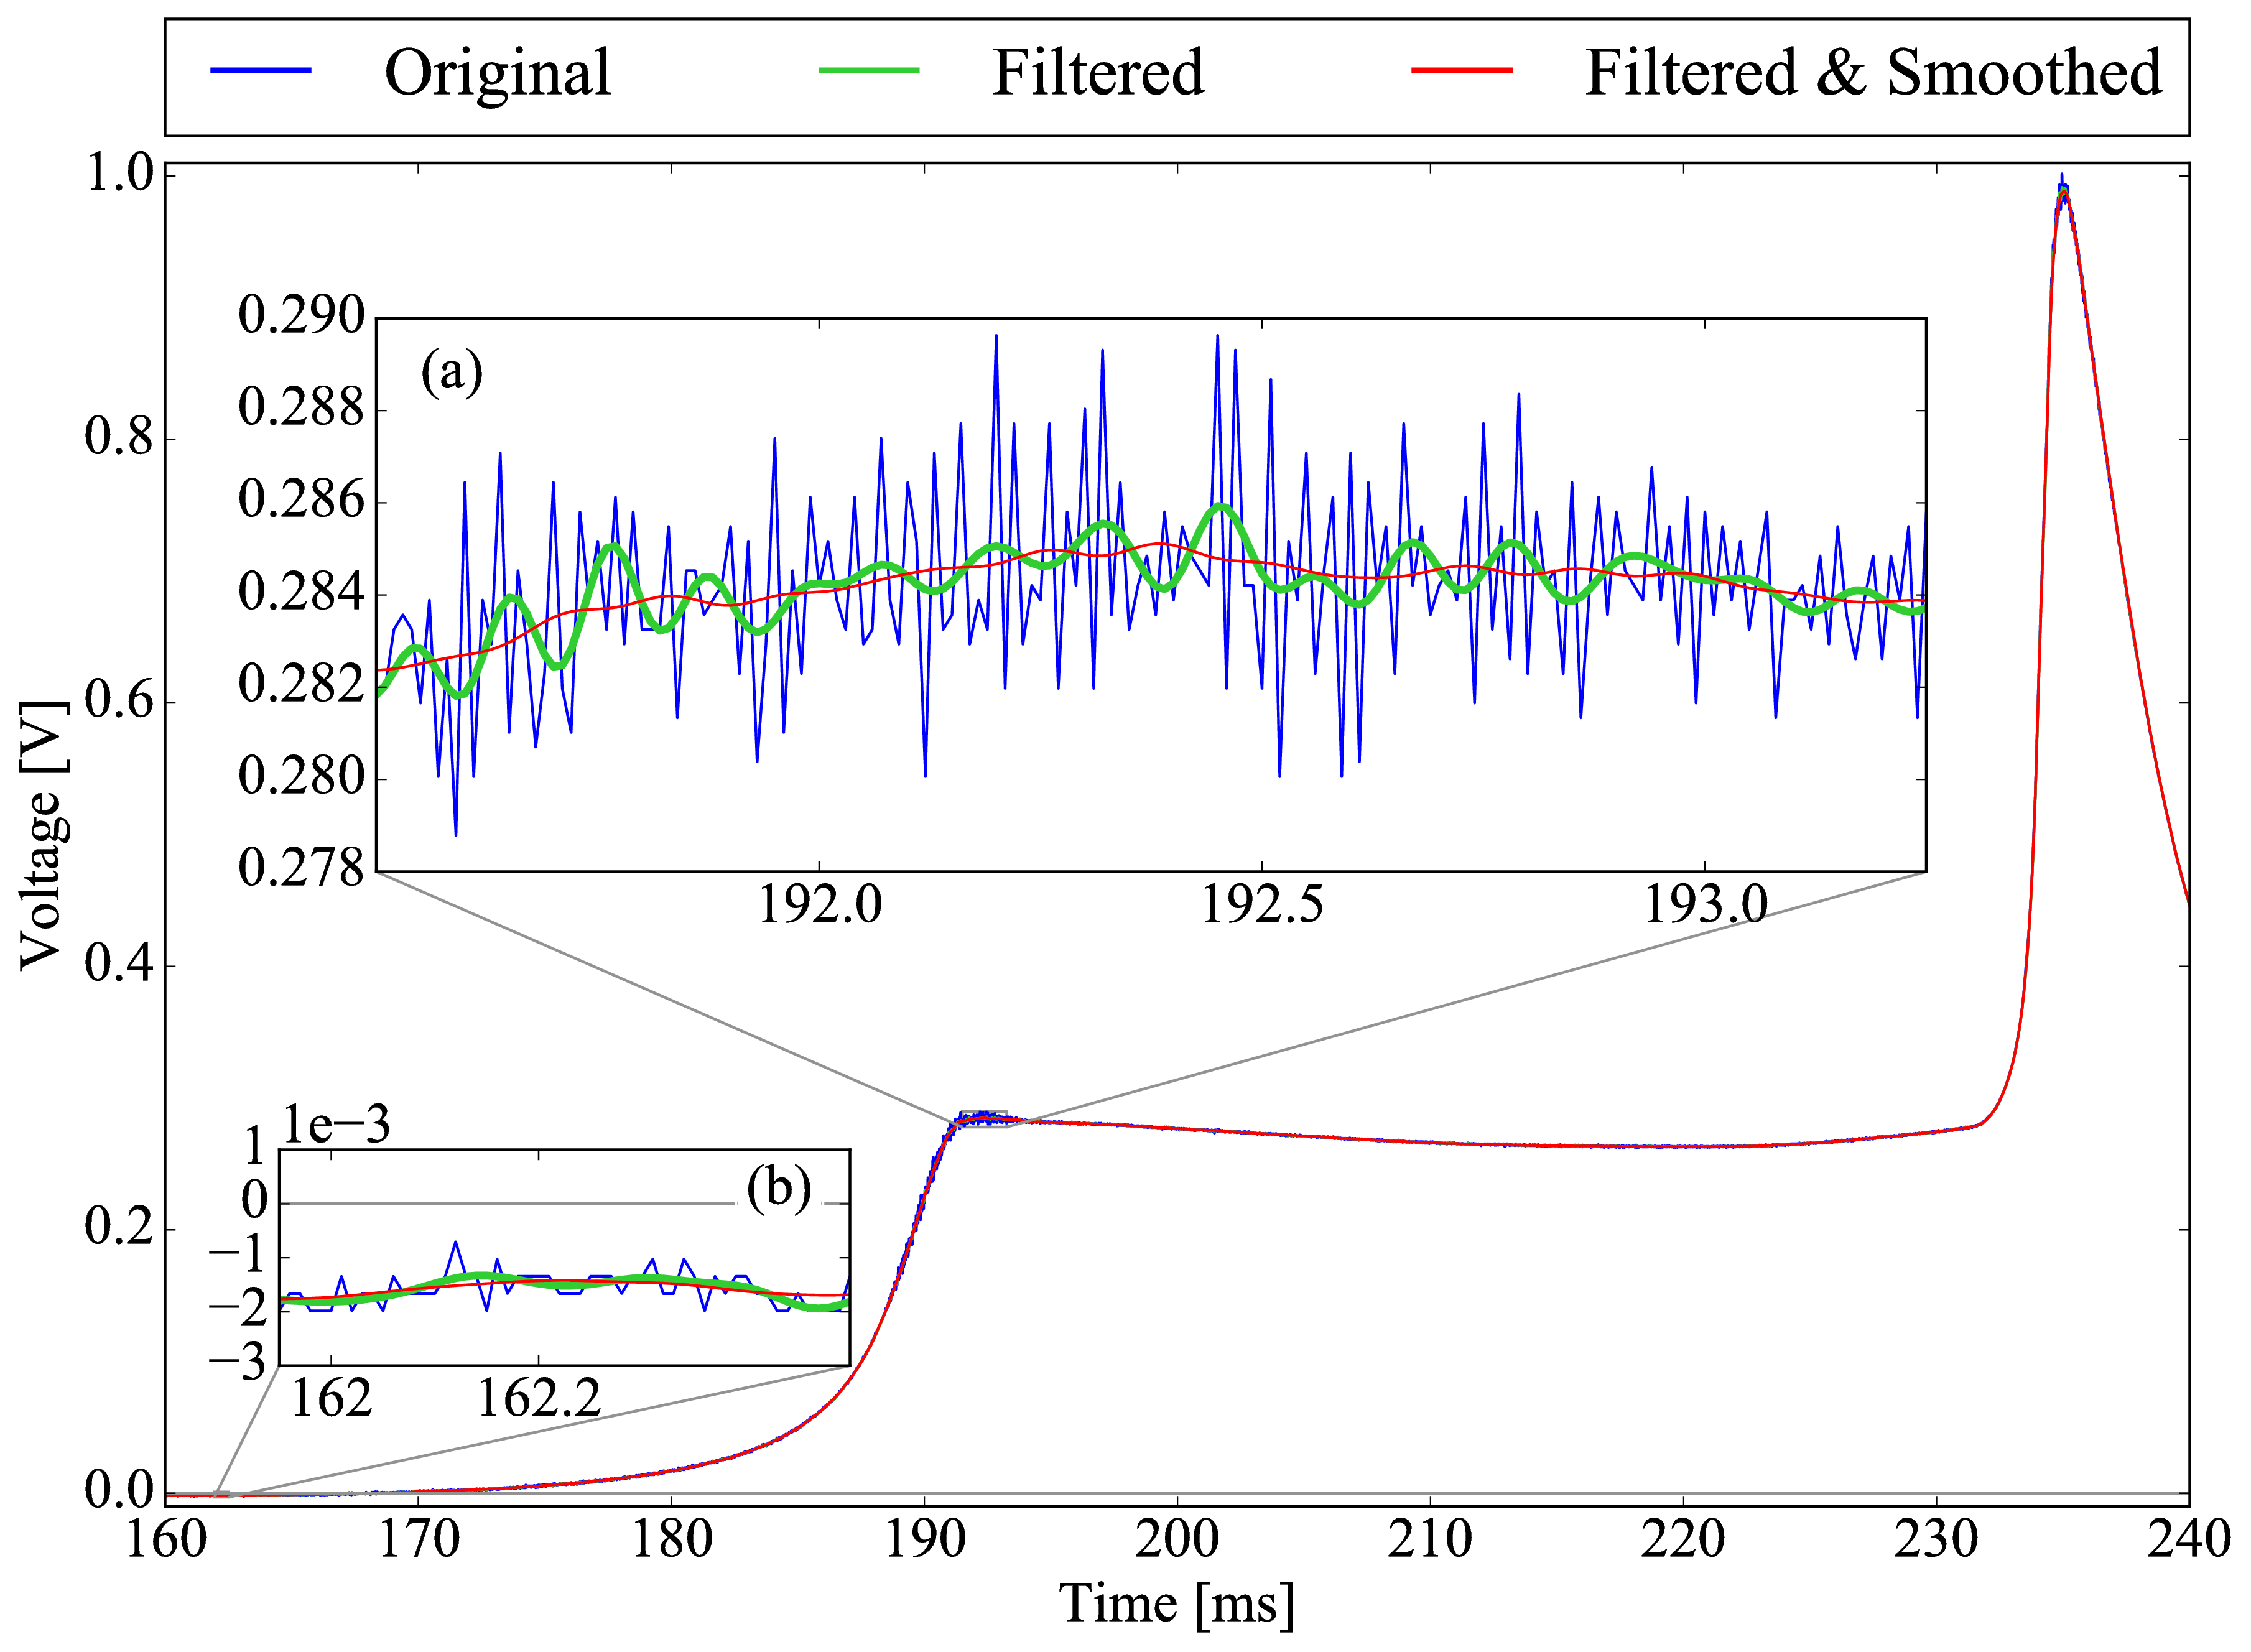
\includegraphics[width=0.75\textwidth]{figures/raw-voltage.png}
\caption{Raw voltage trace and the voltage trace after filtering and
smoothing from a typical RCM experiment. Note that the voltage in the
figure varies from \SIrange{0}{1}{\V} because the scale factor is \SI{100}{\bar\per\V} and
the maximum pressure for this case is near \SI{100}{\bar}. (a): Close up of the
time around the EOC, demonstrating the fidelity of the smoothed and
filtered signal with the original signal. (b): Close up of the time
before the start of compression, demonstrating the offset of the initial
voltage slightly below \SI{0}{\V}.}
\label{fig:raw-voltage}
\end{figure}

\Cref{fig:raw-voltage} shows a typical voltage trace measured from
the RCM at UConn. Several features are apparent from this figure. First,
the compression stroke takes approximately \SIrange{30}{40}{\ms} and
approximately \SI{50}{\percent} of the pressure rise occurs in the last \SI{5}{\ms}of
compression. Second, there is a slow pressure decrease after the EOC due
to heat transfer from the reactants to the relatively colder chamber
walls. Third, after some delay period there is a spike in the pressure
corresponding to rapid heat release due to combustion. Finally, the
signal can be somewhat noisy, requiring filtering and/or smoothing to
produce a useful pressure trace.

\subsection{Filtering and Smoothing}\label{filtering-and-smoothing}

In the current version of UConnRCMPy \autocite{uconnrcmpy}, the voltage
is filtered using a low-pass filter with a cutoff frequency of \SI{10}{\kHz}.
The filter is constructed using the \mintinline{python}|firwin()| function from the
\mintinline{python}|signals| module of SciPy \autocite{Jones2001} with the Blackman
window \autocite{Blackman1958,Oppenheim1999} and a filter
order of \(2^{14}-1\). The cutoff frequency, window type, and filter
order were determined empirically, based on \cref{fig:frequency}. Methods to select a cutoff frequency that
optimizes the signal-to-noise ratio are currently being investigated.

\begin{figure}[htbp]
\centering
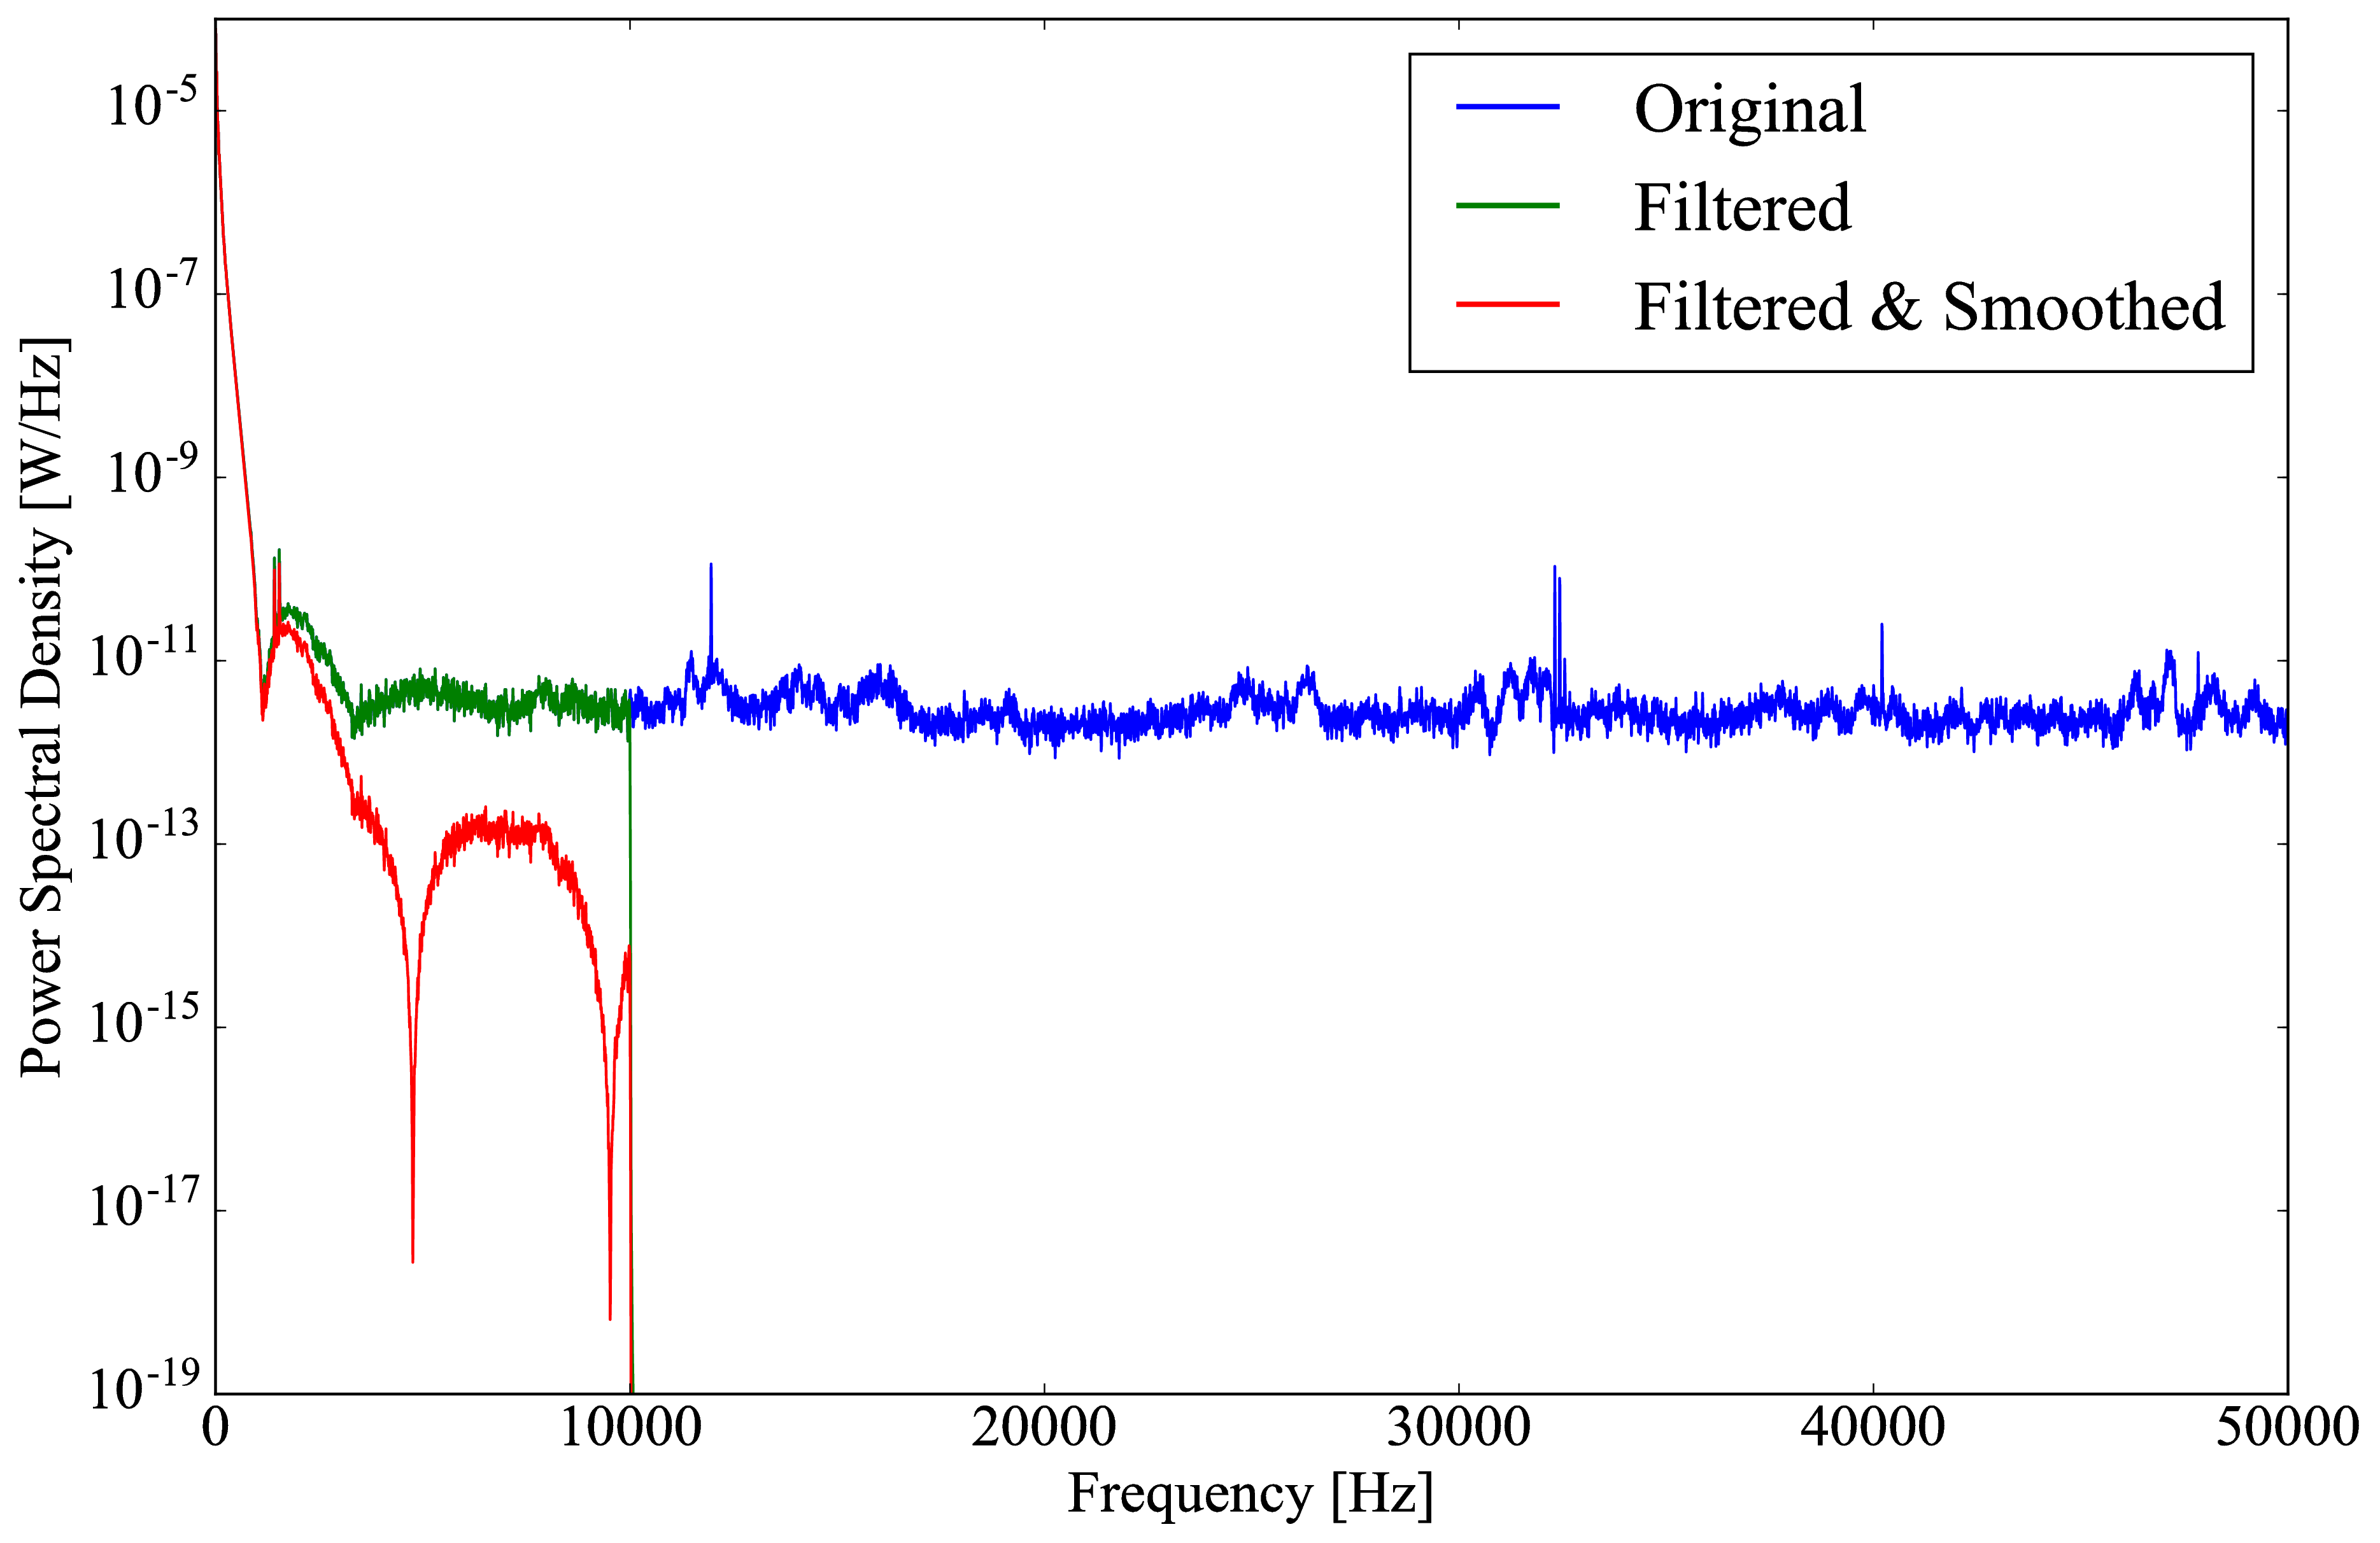
\includegraphics[width=0.9\textwidth]{figures/frequency.png}
\caption{Power spectral density profiles of the original, filtered, and
filtered and smoothed signals, showing the peaks of noise above 10 kHz.}
\label{fig:frequency}
\end{figure}

After filtering, the signal is smoothed by a moving average filter with
a width of 21 points. This width was selected empirically based on
\cref{fig:raw-voltage} to minimize the deviation of the
smoothed voltage from the raw voltage during the ignition, and methods
to automatically choose an optimal width are being investigated. It is
desired that the signal remain the same length through this operation,
but the convolution operation used to apply the moving average zero-pads
the first and last 10 points. To avoid a bias in the initial voltage,
the first 10 points are set equal to the value of the 11th point; the
final 10 points are not important in the rest of the analysis and are
ignored. The result of the filtering and smoothing operations is shown
on \cref{fig:raw-voltage}.

\subsection{Offset Correction and Pressure Calculation}\label{offset-correction-and-pressure-calculation}

In general, the voltage trace can be converted to a pressure trace by
%
\begin{equation}
    P(t) = F \cdot \overline{V}(t) + P_0
\end{equation}
%
where \(\overline{V}(t)\) is the filtered and smoothed voltage trace and
\(F\) is the scale factor from the charge amplifier. However, as can be
seen in \cref{fig:raw-voltage}~b there is a small offset
in the initial voltage relative to the nominal value of \SI{0}{\V}. To correct
for this offset, it can be subtracted from the voltage trace
%
\begin{equation}
    P(t) = F \cdot \left[\overline{V}(t) - \overline{V}(0)\right] + P_0
\end{equation}
%
where \(\overline{V}(0)\) is the initial voltage of the filtered and
smoothed signal. Assuming the noise in the signal has an equal
probability of being above or below the mean voltage, choosing the
initial point (i.e., \(\overline{V}(0)\)) to set the voltage offset is
equivalent to choosing any other point prior to the start of
compression. The result is a vector of pressure values that must be
further processed to determine the time of the EOC and the ignition
delay.

\subsection{Finding the EOC}\label{finding-the-eoc}

In the current version of UConnRCMPy \autocite{uconnrcmpy}, the EOC is
determined by finding the local maximum of the pressure prior to
ignition. This is done by searching backwards in time from the global
maximum pressure in the pressure trace (typically, the global maximum of
the pressure is due to ignition) until a minimum in the pressure is
reached. Since the precise time of the minimum is not important for this
method, the search is done by comparing the pressure at a given index
\(i\) to the pressure at point \(i-50\), starting with the index of the
global maximum pressure. The comparison is not made to the adjacent
point to avoid the influence of noise. If \(P(i) \geq P(i-50)\), the
index is decremented and the process is repeated until
\(P(i) < P(i-50)\). This value of \(i\) is approximately at the minimum
of pressure prior to ignition, so the maximum of the pressure in points
to the left of the minimum will be the EOC.

This method is generally robust, but it fails when there is no minimum
in the pressure between the EOC and ignition, or the minimum pressure is
very close to the EOC pressure. This may be the case for short ignition
delays, on the order of \SI{5}{\ms} or less. In these cases, the comparison
offset (which is set to 50 points by default) can be reduced to improve
the granularity of the search; if the method still fails, manual
intervention is necessary to determine the EOC. In either case, the
value of the pressure at the EOC, \(P_C\), is recorded and the time at
the EOC is taken to be \(t=\SI{0}{\s}\).

\subsection{Calculating Ignition Delay}\label{calculating-ignition-delay}

The ignition delay is determined as the time difference between the EOC
and the point of ignition. There are several definitions of the point of
ignition; the most commonly used in RCM experiments is the inflection
point in the pressure trace due to ignition. As before, finding zero
crossings of the second time derivative of the pressure to define the
inflection point is difficult due to noise; however, finding the maximum
of the first derivative is trivial, particularly since the time before
and shortly after the EOC can be excluded to avoid the peak in the
derivative around the EOC.

In the current version of UConnRCMPy \autocite{uconnrcmpy}, the first
derivative of the experimental pressure trace is computed by a
second-order forward differencing method. The derivative is then
smoothed by the moving average algorithm with a width of 151 points.
This value for the moving average window was chosen empirically.

For some conditions, the reactants may undergo two distinct stages of
ignition. These cases can be distinguished by a pair of peaks in the
first time derivative of the pressure. For some two-stage ignition
cases, the first-stage pressure rise, and consequently the peak in the
derivative, are relatively weak, making it hard to distinguish the peak
due to ignition from the background noise. This is currently the area
requiring the most manual intervention, and one area where significant
improvements can be made by refining the differentiation and
filtering/smoothing algorithms. An experiment that shows two clear peaks
in the derivative is shown in \cref{fig:ign-delay-def} to
demonstrate the definition of the ignition delays.

\begin{figure}[htbp]
\centering
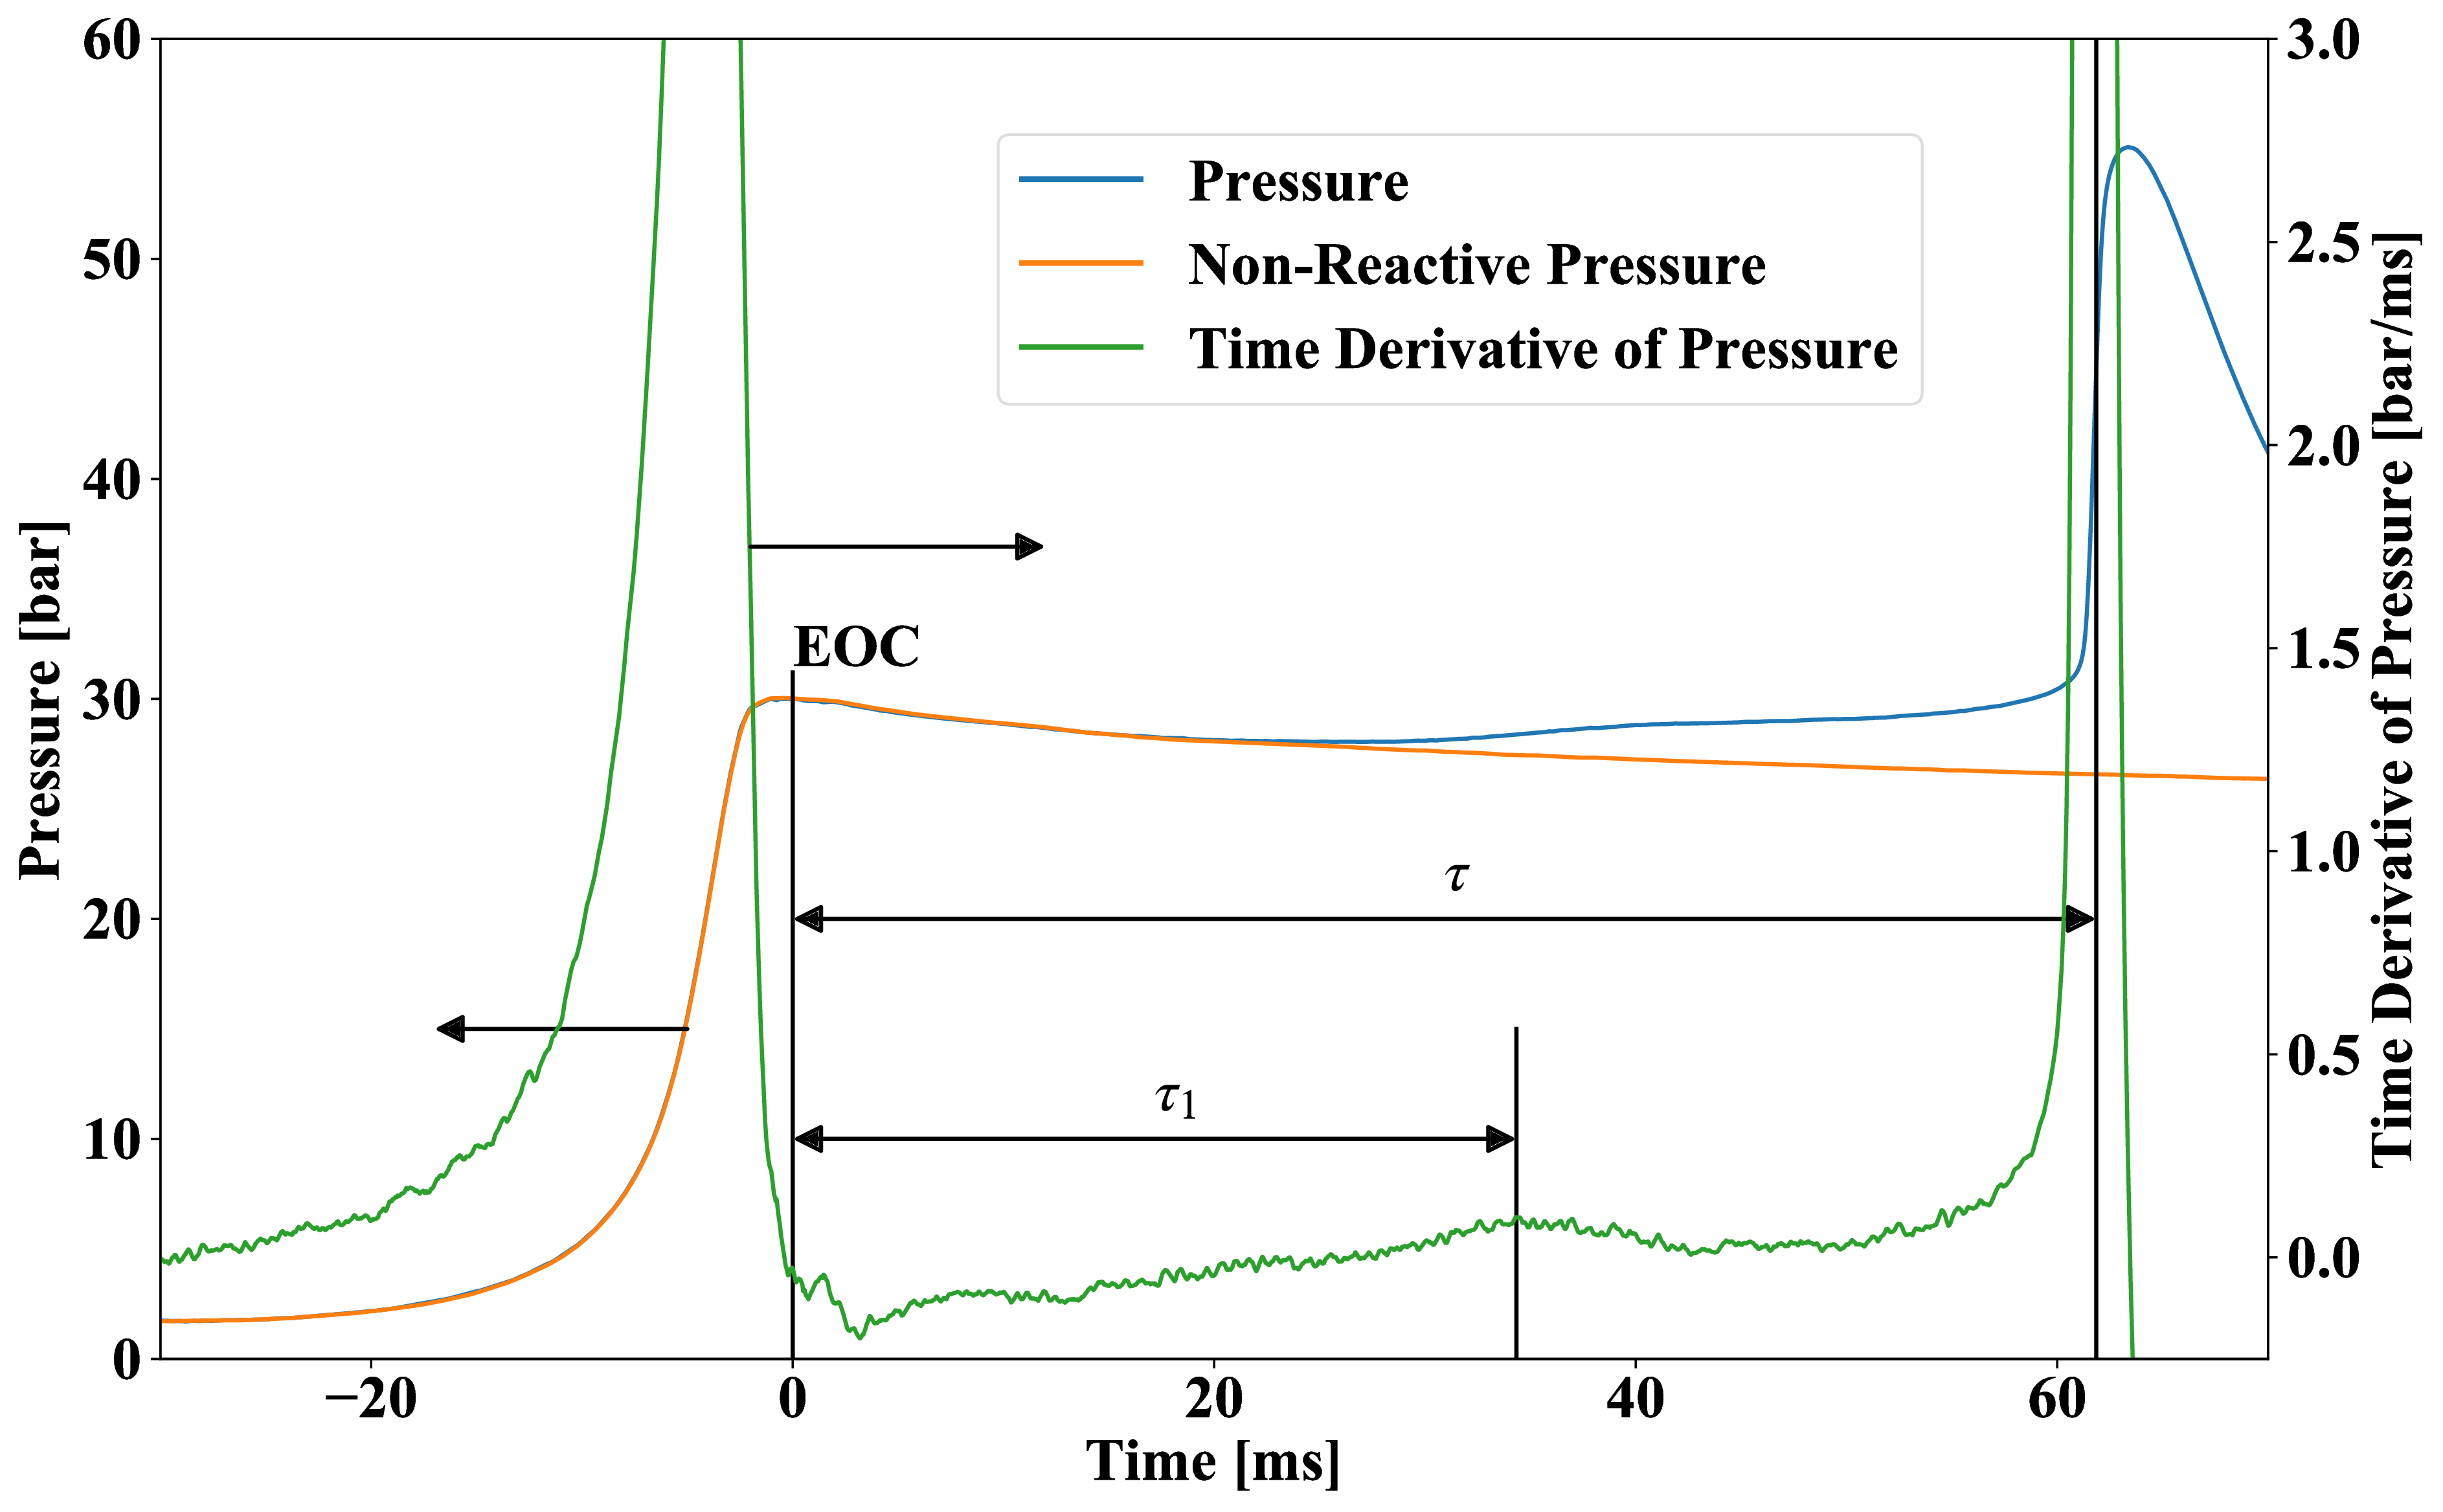
\includegraphics[width=0.9\textwidth]{figures/ign-delay-def.png}
\caption{Illustration of the definition of the ignition delay in a
two-stage ignition case.}
\label{fig:ign-delay-def}
\end{figure}

\subsection{Calculating the EOC Temperature}\label{calculating-the-eoc-temperature}

The final parameter of interest presently is the EOC temperature,
\(T_C\). This temperature is often used as the reference temperature
when reporting ignition delays. In general, it is difficult to measure
the temperature as a function of time in the reaction chamber of the
RCM, so methods to estimate the temperature from the pressure trace are
used.

The law of conservation of energy written for the ideal gases in the
reaction chamber is:
%
\begin{equation} \label{eq:first-law}
    c_v \frac{dT}{dt} = -P \frac{dv}{dt} - \sum_k u_k \frac{d Y_k}{dt}
\end{equation}
%
where \(c_v\) is the specific heat at constant volume of the mixture,
\(v\) is the specific volume, \(u_k\) and \(Y_k\) are the specific
internal energy and mass fraction of the species \(k\), and \(t\) is
time. For a constant-area piston, the rate of change of the volume is
equal to the piston velocity. In UConnRCMPy, \cref{eq:first-law} is
integrated by Cantera \autocite{cantera}.

In Cantera, intensive thermodynamic information about the system is
stored in an instance of the \mintinline{python}|Solution| class. The
\mintinline{python}|Solution| classes used in this study model simple, compressible
systems and require two independent properties, plus the composition, to
fix the state. The two properties must be intensive (i.e., not dependent
on system size), and are typically chosen from the pressure,
temperature, and density. The thermodynamic information for each species
is read from a file in the CTI format, described in the Cantera
documentation \autocite{cantera}, when a \mintinline{python}|Solution| instance is
created.

In addition to evaluating thermodynamic data, Cantera \autocite{cantera}
contains several objects used to model homogeneous reacting systems; the
two used in UConnRCMPy are the \mintinline{python}|Reservoir| and the
\mintinline{python}|IdealGasReactor|, which are subclasses of the generic
\mintinline{python}|Reactor| class. A \mintinline{python}|Solution| object is installed in each
\mintinline{python}|Reactor| subclass instance to manage the state information and
evaluate thermodynamic properties. The difference between the
\mintinline{python}|Reservoir| and the \mintinline{python}|IdealGasReactor| is simply that the
state (i.e., the pressure, temperature, and chemical composition) of the
\mintinline{python}|Solution| in a \mintinline{python}|Reservoir| is fixed.

Integrating \cref{eq:first-law} requires knowledge of the
volume of the reaction chamber as a function of time. To calculate the
volume as a function of time, it is assumed that there is a core of gas
in the reaction chamber that undergoes an isentropic compression
\autocite{Lee1998}. Furthermore, it is assumed that there is negligible
reactant consumption during the compression stroke.

Constructing the volume trace is triggered by the user by running the
\mintinline{python}|create_volume_trace()| method that implements the following
procedure. A Cantera \mintinline{python}|Solution| object is initialized at the
initial temperature, pressure, and composition of the reaction chamber.
After initialization, UConnRCMPy stores the initial mass-specific
entropy (\(s_0\)) and density (\(\rho_0\)). The initial volume is
arbitrarily taken to be \(V_0=\SI{1.0}{\m\cubed}\). The initial volume used
in constructing the volume trace is arbitrary provided that the same
value is used for the initial volume in the simulations described below.
However, extensive quantities such as the total heat release during
ignition cannot be compared to experimental values.

The measured pressure at each point in the pressure trace (\(P_i\)) is
used with the previously recorded initial entropy (\(s_0\)) to set the
state of the \mintinline{python}|Solution| object sequentially. At each point, the
volume is computed by applying the ideal gas law:
%
\begin{equation}
 V_i = V_0 \frac{\rho_0}{\rho_i}
\end{equation}
%
where \(\rho_i\) is the density at each point computed by the Cantera
\mintinline{python}|Solution|. This procedure effects a constant composition
isentropic compression process.

Once the volume trace has been generated, it can be utilized in the
\mintinline{python}|IdealGasReactor| and the solution of \cref{eq:first-law} by installing an instance of the
\mintinline{python}|Wall| class. \mintinline{python}|Wall|s must be installed between instances
of \mintinline{python}|Reactor|s, so in UConnRCMPy a \mintinline{python}|Wall| is installed
between the \mintinline{python}|IdealGasReactor| that represents the reaction
chamber and an instance of the \mintinline{python}|Reservoir| class. By specifying
the velocity of the \mintinline{python}|Wall| using the volume trace, the
\mintinline{python}|IdealGasReactor| will proceed through the same states as the
reaction chamber in the experiment. The velocity of the \mintinline{python}|Wall| is
specified by using an instance of the \mintinline{python}|VolumeProfile| class from
the CanSen software \autocite{cansen}, which computes the first forward
difference of the volume as a function of time.

Finally, the \mintinline{python}|IdealGasReactor| is installed into an instance of
\mintinline{python}|ReactorNet| from Cantera \autocite{cantera}. The
\mintinline{python}|ReactorNet| implements the interface to the solver CVODES.
CVODES is an adaptive-time-stepping ODE solver, distributed as part of the
SUNDIALS suite \autocite{Hindmarsh2005}.

Two simulations can be triggered by the user that utilize this
procedure. In the first, the multiplier for all the reaction rates is
set to zero, to simulate a constant composition (non-reactive) process.
In the second, the reactions are allowed to proceed as normal. Only the
non-reactive simulation is necessary to determine \(T_C\), which is
defined as the simulated temperature at the EOC time.

When a reactive simulation is conducted, the user must compare the
temperature traces from the two simulations to verify that the inclusion
of the reactions does not change \(T_C\), validating the assumption of
adiabatic, constant composition compression. Although including
reactions during the compression stroke does not affect the value of
\(T_C\), it does allow for the buildup of a small pool of radicals that
can affect processes after the EOC \autocite{Mittal2008}. Thus, it is
critical to include reactions during the compression stroke when
conducting simulations to compare a kinetic model to experimental
results.

\subsection{Simulating Post-EOC Processes}\label{simulating-post-eoc-processes}

As can be seen in \cref{fig:ign-delay-def}, the pressure
decreases after the EOC due to heat transfer from the higher temperature
reactants to the reaction chamber walls. This process is specific to the
machine that carried out the experiments, and to the conditions under
which the experiment was conducted. Therefore, the rate of pressure
decrease should be modeled and included in simulations that compare
predicted ignition delays to the experimental values.

To conduct this modeling, a non-reactive experiment is conducted, where
\(\text{O}_2\) in the oxidizer is replaced with \(\text{N}_2\) to
maintain a similar specific heat ratio but suppress the oxidation
reactions that lead to ignition. The pressure trace from this
non-reactive experiment should closely match that from the reactive
experiment during the compression stroke, further validating the
assumption of adiabatic, constant composition compression. Furthermore,
the non-reactive pressure trace should closely match the reactive
pressure trace after the EOC until exothermic reactions cause the
pressure in the reactive experiment to begin to increase.

To apply the effect of the post-compression heat loss into the
simulations, the reaction chamber is modeled as undergoing an adiabatic
volume expansion. Since the post-compression time is modeled as an
isentropic expansion, the same procedure is used as in the computation
of \(T_C\) to compute a volume trace for the post-EOC time. The only
difference is that the non-reactive pressure trace is used after the EOC
instead of the reactive pressure trace. Once the volume trace is
generated, it can be applied to a simulation by concatenating the volume
trace of the compression stroke and the post-EOC volume trace together
and following the procedure outlined in \cref{calculating-the-eoc-temperature}.
For consistency, the ignition delay in a reactive
simulation is defined in the same manner as in the reactive experiments,
as the maxima of the time derivative of the pressure trace. This
procedure has been validated experimentally by measuring the temperature
in the reaction chamber during and after the compression stroke. The
temperature of the reactants was found to be within $\pm\sim $\SI{5}{\K} of the
simulated temperature \autocite{Das2012a,Uddi2012}.

\section{Implementation of
UConnRCMPy}\label{implementation-of-uconnrcmpy}

UConnRCMPy is constructed in a hierarchical manner. The main user
interface to UConnRCMPy is through the \mintinline{python}|Condition| class, the
highest level of data representation. The \mintinline{python}|Condition| class
contains all of the information pertaining to the experiments at a given
condition. The intended use of this class is in an interactive Python
interpreter (the author prefers the Jupyter Notebook with an IPython
kernel \autocite{Perez2007}). \mintinline{python}|Condition| also contains all the
methods that make up the user interface:

\begin{itemize}
\item
  \mintinline{python}|add_experiment()|
\item
  \mintinline{python}|create_volume_trace()|
\item
  \mintinline{python}|compare_to_sim()|
\end{itemize}

The usage of these methods will be described in detail in the
\href{usage-example}{Usage Example} section. In general, the user will
conduct several experiments and, using the \mintinline{python}|add_experiment()|
method, will trigger UConnRCMPy to create instances of the
\mintinline{python}|Experiment| class and extract the ignition delay.

All of the information about a particular experimental run is stored in
the \mintinline{python}|Experiment| class. When initialized, the \mintinline{python}|Experiment|
expects an instance of the \mintinline{python}|pathlib.Path| class; if none is
provided, it prompts the user to enter a file name that is expected to
be in the current working directory. The file name should point to a
tab-delimited plain text file that contains the voltage trace recorded
by LabView from one experimental run. Then UConnRCMPy creates an
instance of \mintinline{python}|VoltageTrace|, followed by an instance of
\mintinline{python}|ExperimentalPressureTrace|. The pressure trace from the latter
is processed to extract the ignition delay(s).

The lowest level representation of data in UConnRCMPy is the
\mintinline{python}|VoltageTrace| that contains the raw voltage signal and timing
recorded from the DAQ, as well as the filtered and smoothed voltage
traces. The filtering and smoothing algorithms are implemented as
separate methods so they can be reused in other situations and are run
automatically when the \mintinline{python}|VoltageTrace| is initialized.

One step up from the \mintinline{python}|VoltageTrace| is the
\mintinline{python}|ExperimentalPressureTrace| class. This class consumes a
\mintinline{python}|VoltageTrace| and processes it into a pressure trace, given the
multiplication factor from the charge amplifier and the initial
pressure. This class also contains methods to compute the derivative of
the experimental pressure trace, as discussed in
\cref{calculating-ignition-delay}.

When all the experiments are conducted and processed,
\mintinline{python}|create_volume_trace()| further processes the experiments to
create the volume trace necessary to run the simulations to determine
\(T_C\). The actual computation of the volume trace is done by the
\mintinline{python}|VolumeFromPressure| class. First, the volume trace of the
pre-EOC portion is generated using the pre-EOC pressure trace, the
experimental initial temperature, and an initial volume of
\(V_0=\SI{1.0}{\m\cubed}\), as discussed in
\cref{calculating-the-eoc-temperature}.
A temperature trace is also constructed for the pre-EOC pressure trace
using the \mintinline{python}|TemperatureFromPressure| class.

For the post-EOC volume trace, the initial temperature is estimated as
the final value of the temperature trace constructed for the pre-EOC
period. Furthermore, the initial volume of the post-EOC volume trace is
taken to be the final value of the pre-EOC volume trace, so that
although there may be small mismatches in \(P_C\), the volume trace will
be consistent.

After generation, \mintinline{python}|create_volume_trace()| writes the volume
trace out to a CSV file so that the volume trace can be used in other
software. The reactive pressure trace is also written to a tab-separated
file. Before writing, the volume and pressure traces are both
downsampled by a factor of 5. This reduces the computational time of a
simulation and does not have any effect on the simulated results.
\mintinline{python}|create_volume_trace()| also generates a figure that plots the
complete reactive pressure trace, a non-reactive pressure trace
generated from the volume trace using the \mintinline{python}|PressureFromVolume|
class, and a linear fit to the constant pressure period prior to the
start of compression. This linear fit aids in determining a suitable
compression time. Finally, the value of the pressure at the beginning of
compression is put on the system clipboard to be pasted into a
spreadsheet to record the \(P_0\) used for simulations. This may differ
slightly from the \(P_0\) read from the static transducer due to noise
in the signal.

The final step is to use the volume trace in a simulation to determine
\(T_C\). To begin the simulations, the user calls the
\mintinline{python}|compare_to_sim()| method of the \mintinline{python}|Condition|. The
\mintinline{python}|compare_to_sim()| method relies on the
\mintinline{python}|run_simulation()| method, which in turn adds instances of the
class \mintinline{python}|Simulation| to the \mintinline{python}|Condition| instance. Instances
of \mintinline{python}|Simulation| can represent a reactive or a non-reactive
experiment; if either type of simulation has already been added to the
\mintinline{python}|Condition| instance, the user is asked whether they would like
to overwrite the existing simulation.

The \mintinline{python}|Simulation| class sets up the simulation in Cantera and
importantly, sets the maximum time step to be the time step used in the
volume trace, so that the solver does not take steps larger than the
resolution of the velocity. Larger time steps may result in incorrect
calculation of the state if the velocity is not properly applied to the
reactor. The time, temperature, pressure, and simulated volume are
stored in NumPy arrays \autocite{vanderWalt2011} and the derivative is
computed using second order Lagrange polynomials, as suggested by Chapra
and Canale \autocite{Chapra2010} because the time step is not constant
in the simulation. Finally, the calculated value of \(T_C\) is placed
into the system clipboard. If the reactive simulation is conducted, the
overall ignition delay is also copied into the system clipboard. The
first stage ignition delay must be found manually because determining
peaks in the derivative is currently unreliable, as mentioned in
\cref{calculating-ignition-delay} for experiments.

The \mintinline{python}|compare_to_sim()| method also plots the experimental
pressure trace and any of the simulated pressure traces that have been
generated. If the simulated reactive pressure trace is generated, the
time derivative of the pressure is also plotted, where the derivative is
scaled by the maximum pressure in the reactive simulation.

\begin{figure}[htbp]
\centering
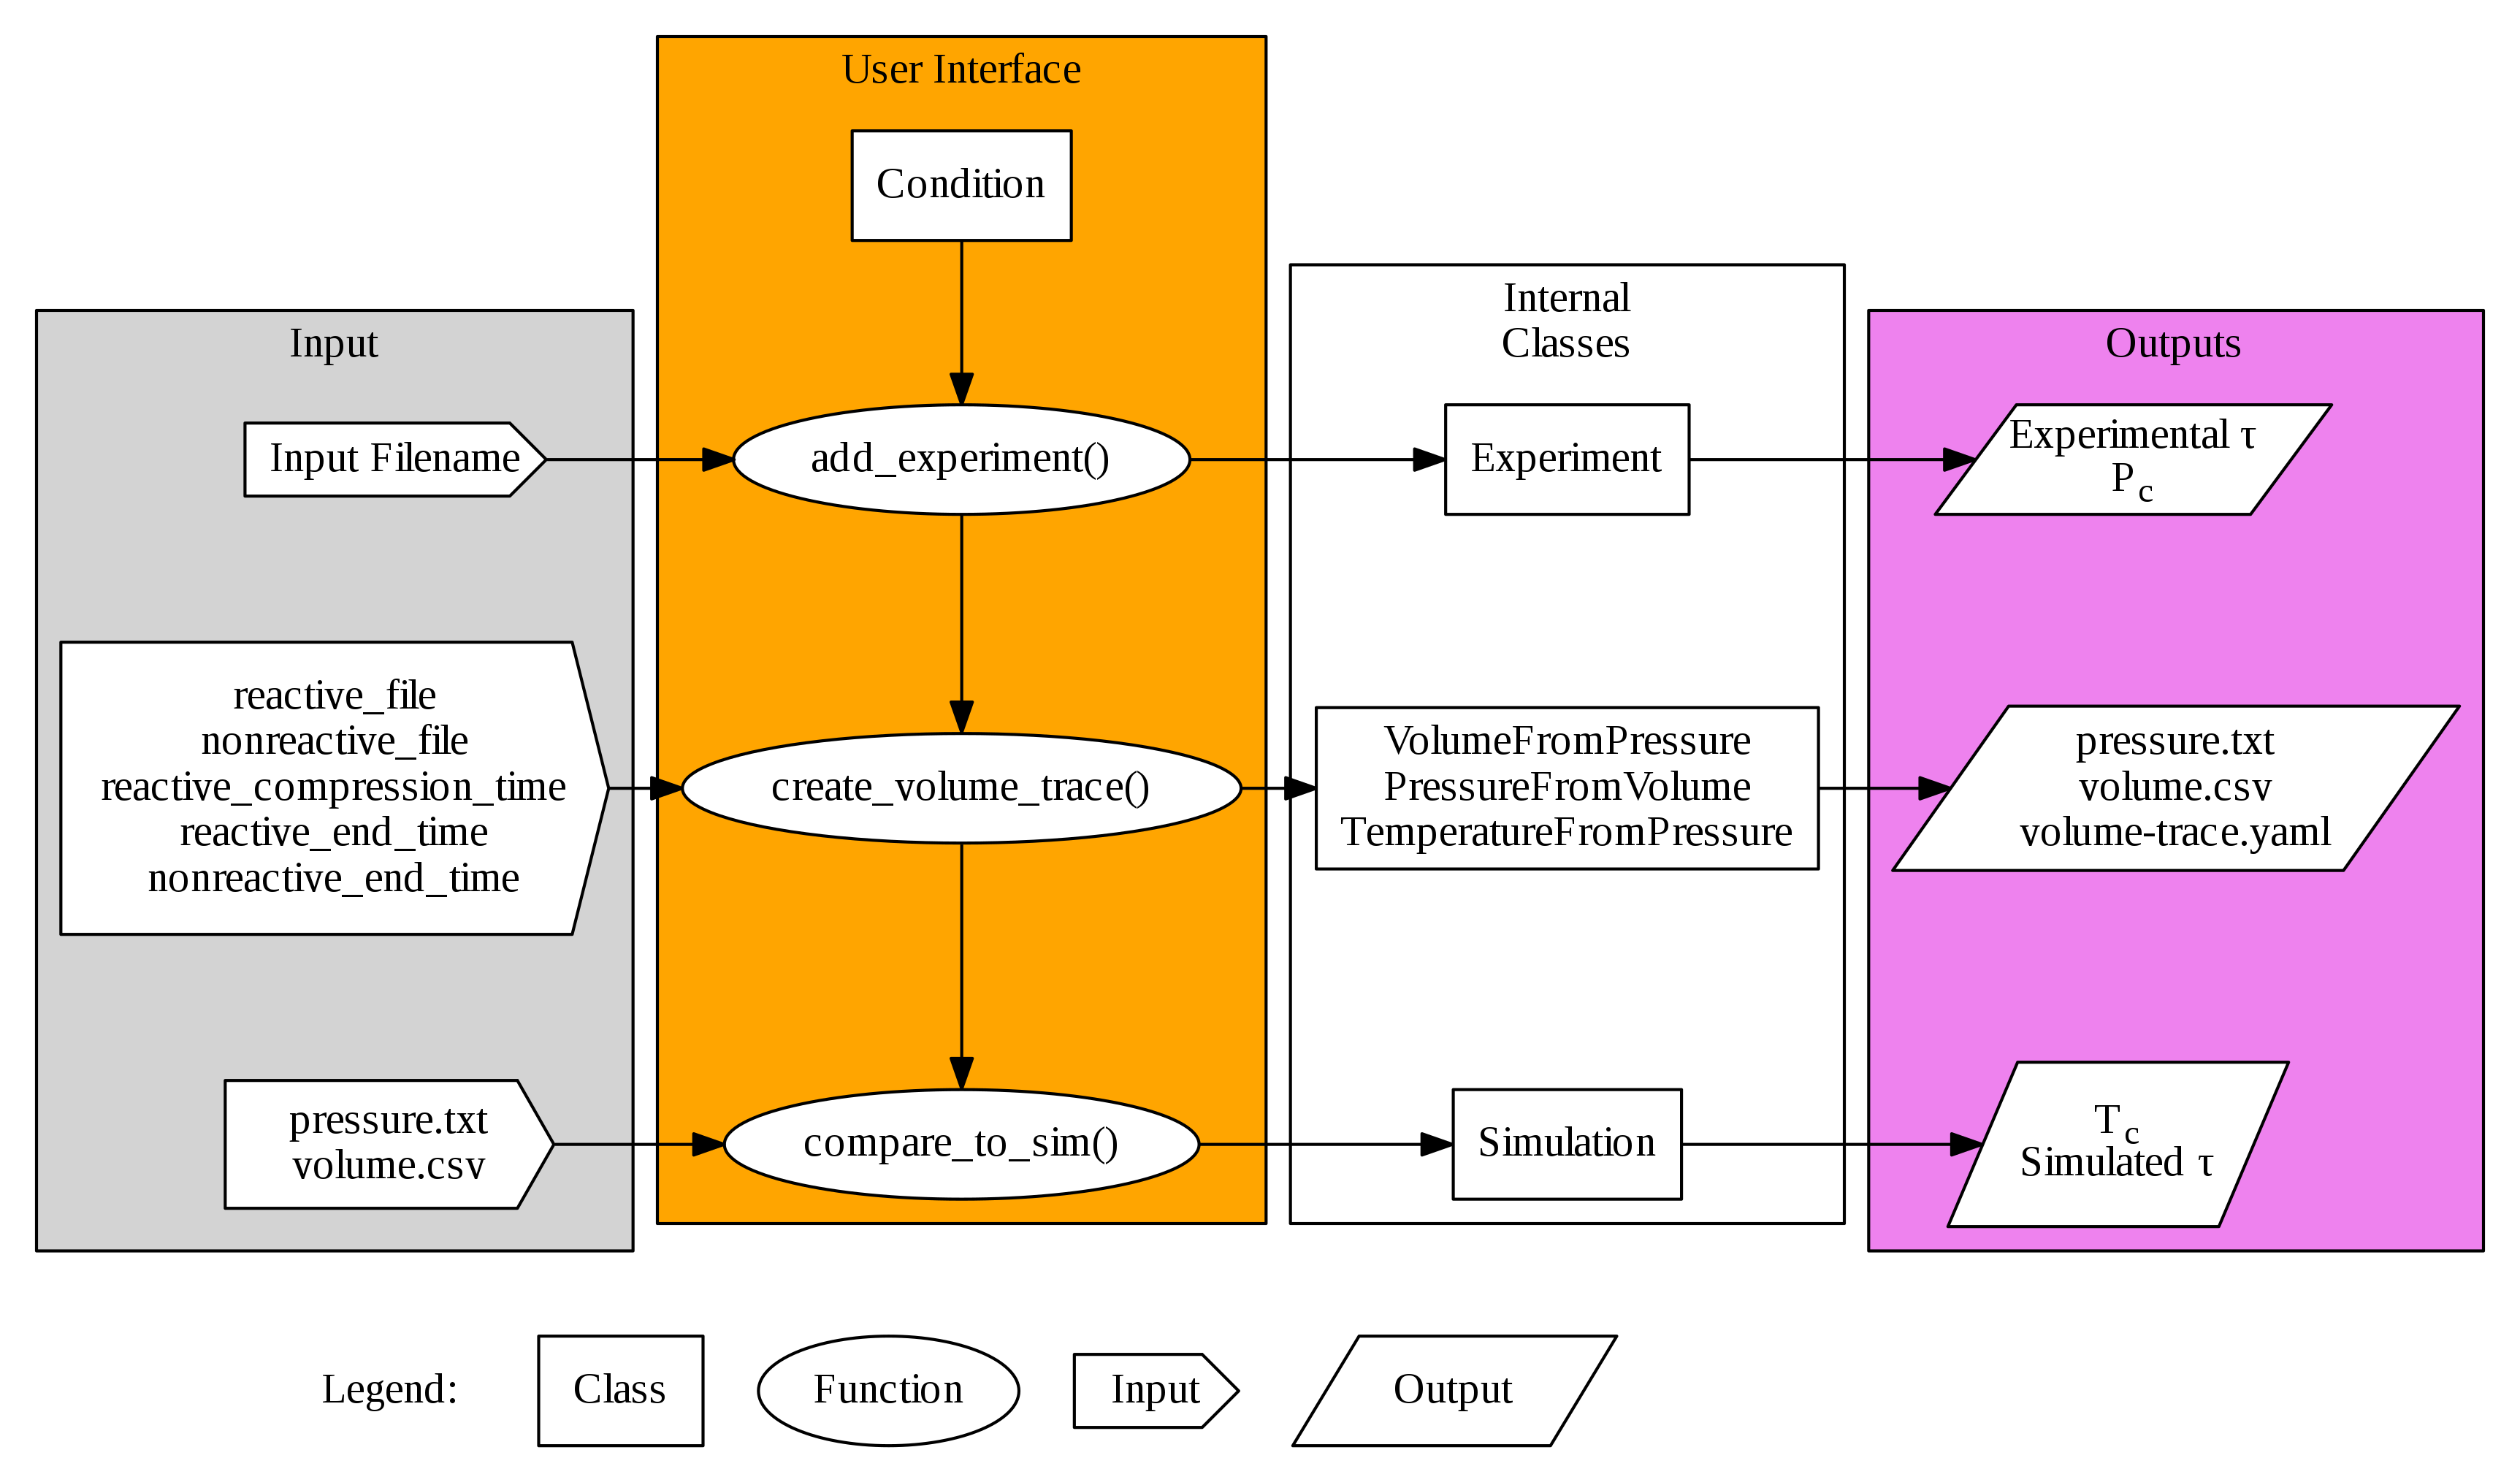
\includegraphics[width=0.9\textwidth]{figures/flowchart.png}
\caption{Flowchart of information in UConnRCMPy.}
\label{fig:flowchart}
\end{figure}

The general flow of the user interaction with UConnRCMPy is shown in
\cref{fig:flowchart}. The Inputs are required input from the
user, while the User Interface are classes and functions called by the
user during processing.

UConnRCMPy is documented using standard Python docstrings for functions
and classes. The documentation is converted to HTML files by the Sphinx
documentation generator \autocite{Brandl2016}. The format of the
docstrings conforms to the NumPy docstring format so that the autodoc
module of Sphinx can be used. The documentation is available on the web
at \href{https://bryanwweber.github.io/UConnRCMPy/}.

\section{Usage Example}\label{usage-example}

In the following, two examples of using UConnRCMPy are given, first with
the standard interface and second utilizing a slightly modified
interface corresponding to a different data format. Both examples assume
the user is running in a Jupyter Notebook with an IPython kernel.

\subsection{Standard Interface}\label{standard-interface}

These experiments were conducted with mixtures of propane, oxygen, and
nitrogen \autocite{Dames2016}. The CTI file necessary to run this
example can be found in the Supplementary Material of the work by Dames
et al. \autocite{Dames2016}. It must be named exactly
\mintinline{python}|species.cti| and placed in the current working directory. Then,
the composition of the mixture under consideration must be added to the
\mintinline{python}|initial_state| parameter of the \mintinline{python}|ideal_gas()| method:

\begin{minted}{python}
ideal_gas(
        name='gas',
        elements=...,
        species=...,
        reactions='all',
        initial_state=state(
            temperature=300.0, pressure=OneAtm,
            mole_fractions=(
                'C3H8:0.0403,O2:0.1008,N2:0.8589')))
\end{minted}

Ellipses indicate input that was truncated to save space; the truncated
input is present in the file available with the work of \textcite{Dames2016}. The
initial temperature and pressure are arbitrary, since those are set
based on information stored in the filename of the experiment, but the
\mintinline{python}|mole_fractions| must be set to the appropriate values. The
condition in this example is for a fuel rich mixture, with a target
\(P_C\) of 30 bar. The user creates the \mintinline{python}|Condition|, then
conducts a reactive experiment with the RCM and adds the experiment to
the \mintinline{python}|Condition| using the \mintinline{python}|add_experiment()| method. This
method creates an instance of class \mintinline{python}|Experiment| for each
experiment passed in. As each experiment is processed by UConnRCMPy, the
information from that run is added to the system clipboard for pasting
into some spreadsheet software. In the current version, the information
copied is the time of day of the experiment, the initial pressure, the
initial temperature, the pressure at the EOC, the overall and first
stage ignition delays, an estimate of the EOC temperature, and some
information about the compression ratio of the reactor. This process is
repeated 5 times to ensure repeatable data is obtained.

\begin{minted}{python}
from uconnrcmpy import Condition
from pathlib import Path
%matplotlib

cond_00_in_02_mm = Condition()
# Conduct reactive experiment #1 on the RCM
cond_00_in_02_mm.add_experiment(Path(
    '00_in_02_mm_373K-1285t-100x-19-Jul-15-1620.txt'))
# Conduct reactive experiment #2 on the RCM
cond_00_in_02_mm.add_experiment(Path(
    '00_in_02_mm_373K-1282t-100x-19-Jul-15-1626.txt'))
# Conduct reactive experiment #3 on the RCM
cond_00_in_02_mm.add_experiment(Path(
    '00_in_02_mm_373K-1282t-100x-19-Jul-15-1633.txt'))
# Conduct reactive experiment #4 on the RCM
cond_00_in_02_mm.add_experiment(Path(
    '00_in_02_mm_373K-1282t-100x-19-Jul-15-1640.txt'))
# Conduct reactive experiment #5 on the RCM
cond_00_in_02_mm.add_experiment(Path(
    '00_in_02_mm_373K-1282t-100x-19-Jul-15-1646.txt'))
\end{minted}

This sequence generates one figure showing all of the experiments
together and one figure per experiment comparing the pressure and the
time derivative of the pressure. Matplotlib is used for plotting
\autocite{Hunter2007}. The plots are optional, and are controlled by
passing a boolean keyword argument \mintinline{python}|plotting| when the
\mintinline{python}|Condition| is initialized. The figures showing each experiment
look similar to \cref{fig:ign-delay-def}, but the non-reactive
trace is not plotted and the EOC and ignition delays are not labeled.

In general, for a given condition, the user will conduct and process all
of the reactive experiments before conducting any non-reactive
experiments. Then, the user chooses one of the reactive experiments as
the reference experiment for the condition (i.e., the one whose ignition
delay(s) and \(T_C\) are reported) by inspection of the data in the
spreadsheet. The reference experiment is defined as the experimental run
whose overall ignition delay is closest to the mean overall ignition
delay among the experiments at a given condition. To select the
reference experiment, the user puts the file name of the reference
experiment into a YAML format file called \mintinline{python}|volume-trace.yaml|
with the key \mintinline{python}|reacfile|. For this case, the reference experiment
is the run that took place at 16:33:

\begin{minted}{python}
reacfile: '00_in_02_mm_373K-1282t-100x-19-Jul-15-1633.txt'
\end{minted}

Note that the file must be named exactly \mintinline{python}|volume-trace.yaml| and
it must be located in the current working directory. Once the reference
reactive experiment is selected, the user runs non-reactive experiments
at the same initial conditions as the reference experiment. The user
adds non-reactive experiments to the \mintinline{python}|Condition| by the same
\mintinline{python}|add_experiment()| method and UConnRCMPy automatically
determines whether the experiment is reactive or non-reactive.

\begin{figure}[htbp]
\centering
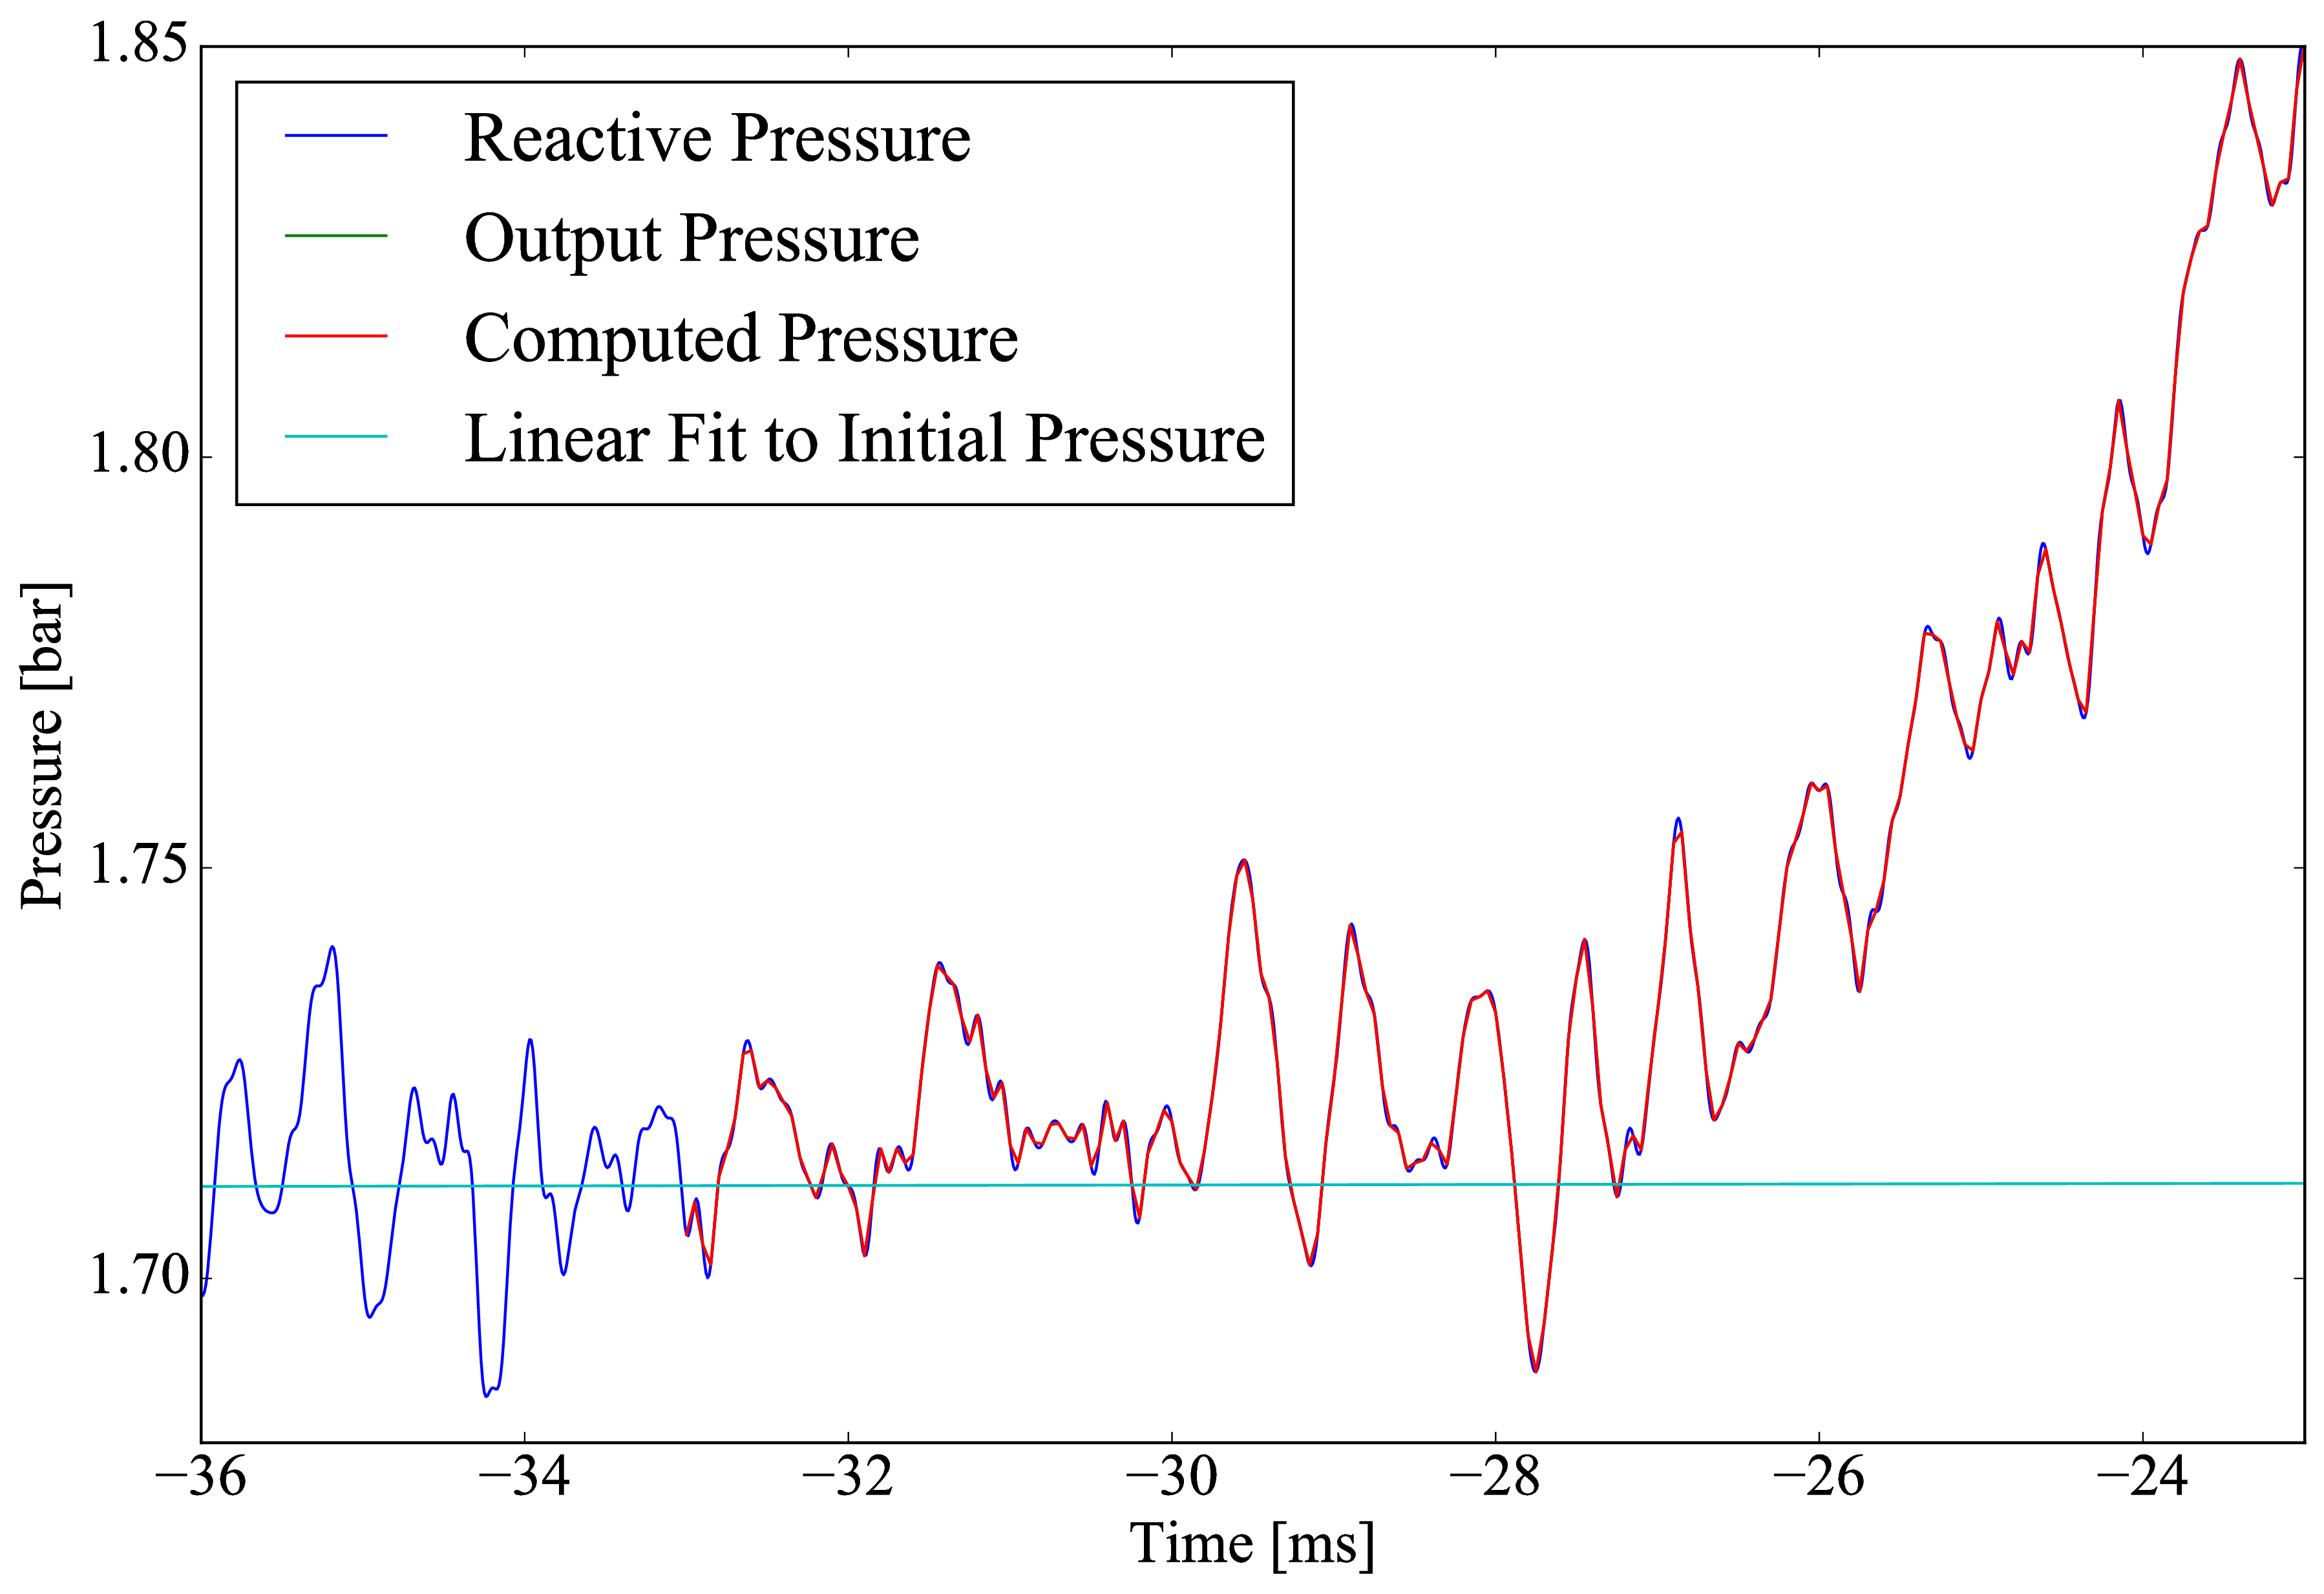
\includegraphics[width=0.9\textwidth]{figures/pressure-comparison.png}
\caption{Comparison of the reactive pressure trace, the pressure trace
output to the text file, the pressure trace computed from the volume
trace, and the linear fit to the initial pressure demonstrating the
choice of compression time. The dark blue, green, and red lines follow
each other nearly exactly after the start of compression, so only the
red line is visible. This is the desired result, indicating that the
pressure traces agree.}
\label{fig:pressure-comparison}
\end{figure}

\begin{minted}{python}
# Conduct non-reactive experiment #1 on the RCM
cond_00_in_02_mm.add_experiment(Path(
'NR_00_in_02_mm_373K-1278t-100x-19-Jul-15-1652.txt'))
\end{minted}

UConnRCMPy determines that this is a non-reactive experiment and
generates a new figure that compares the current non-reactive case with
the reference reactive case as specified in \mintinline{python}|volume-trace.yaml|.
If the user adds a non-reactive experiment before creating the
\mintinline{python}|volume-trace.yaml| file, or if the file referenced in the
\mintinline{python}|reacfile| key is not present in the current working directory,
UConnRCMPy raises a \mintinline{python}|FileNotFound| exception. For this particular
example, the pressure traces are shown in \cref{fig:ign-delay-def}. In this case, the non-reactive
pressure agrees very well with the reactive pressure and no further
experiments are necessary; in principle, any number of non-reactive
experiments can be conducted and added to the figure for comparison.
Since there is good agreement between the non-reactive and reactive
pressure traces, the user adds the non-reactive reference file name to
\mintinline{python}|volume-trace.yaml|.

\begin{minted}{python}
reacfile: '00_in_02_mm_373K-1282t-100x-19-Jul-15-1633.txt'
nonrfile: NR_00_in_02_mm_373K-1278t-100x-19-Jul-15-1652.txt'
comptime: 10
\end{minted}

Then, the user specifies the rest of the parameters in
\mintinline{python}|volume-trace.yaml|, including the compression time and the end
times for the reactive and non-reactive experiments. The reactive end
time (\mintinline{python}|reacend|) determines the length of the output pressure
trace, while the non-reactive end time (\mintinline{python}|nonrend|) determines the
length of the volume trace. The length of the volume trace is also
determined by the compression time (\mintinline{python}|comptime|), which should be
set to a time such that the starting point is before the beginning of
the compression. All three times should be specified in milliseconds.
\mintinline{python}|comptime| is determined by comparison with the fit to the
initial pressure, as shown in \cref{fig:pressure-comparison}.
In this case, the compression has started at approximately
\(t > \SI{-28}{ms}\). The time prior to that where the pressure
appears to stabilize around the initial pressure is approximately
\(t = \SI{-33}{ms}\), giving a compression time of \SI{33}{\ms}.
\mintinline{python}|reacend| is typically chosen to be shortly after the main
pressure peak due to ignition, about \SI{80}{\ms} in this case, and
\mintinline{python}|nonrend| is typically chosen to be \SI{400}{\ms}.

\begin{minted}{yaml}
reacfile: 00_in_02_mm_373K-1282t-100x-19-Jul-15-1633.txt
nonrfile: NR_00_in_02_mm_373K-1278t-100x-19-Jul-15-1652.txt
comptime: 33
nonrend: 400
reacend: 80
\end{minted}

This sample represents a complete, minimal example of the necessary
information in the \mintinline{python}|volume-trace.yaml| file. In addition, two
optional parameters can also be specified in \mintinline{python}|volume-trace.yaml|.
These are offset parameters used to control the precise point where the
switch from the reactive pressure trace to the non-reactive pressure
trace occurs in the volume trace. These parameters may be necessary if
the determination of the EOC does not result in aligned compression
strokes for the reactive and non-reactive experiments, but they are not
generally necessary.

Once the \mintinline{python}|volume-trace.yaml| file is completed, the
\mintinline{python}|create_volume_trace()| method can be run. Then, the final step
is to conduct the simulations to calculate \(T_C\) and the simulated
ignition delay. This is done by the user by running the
\mintinline{python}|compare_to_sim()| function. This function takes two optional
arguments, \mintinline{python}|run_reactive()| and \mintinline{python}|run_nonreactive()|,
both of which are booleans. These determine which type of simulation
should be conducted; by default, \mintinline{python}|run_reactive()| is
\mintinline{python}|False| and \mintinline{python}|run_nonreactive()| is \mintinline{python}|True| because
the reactive simulations may take substantial time (\SI{5}{\min}).
There is no restriction on combinations of values for the
arguments; either or both may be \mintinline{python}|True| or \mintinline{python}|False|.

\begin{minted}{python}
cond_00_in_02_mm.create_volume_trace()
cond_00_in_02_mm.compare_to_sim(
    run_reactive=True,
    run_nonreactive=True,
)
\end{minted}

At this point, the user has completed one experimental condition. Now,
further conditions should be studied, either by changing \(T_0\) or the
compression ratio of the RCM to reach a different value of \(T_C\) for a
given \(P_C\).

\subsection{Modified Interface}\label{modified-interface}

It is also possible to replace parts of the processing interface by
using the features of Python to overload class methods. Due to the
modular nature of UConnRCMPy, small parts of the interface can be
replaced without sacrificing consistent analysis for the critical parts
of the code, such as computing the ignition delay. For instance, ongoing
work involves processing RCM data collected by several operators of the
RCM. Each user has their own file naming strategy that must be parsed
for information about the experiment. To process this ``alternate'' data
format, two new classes called \mintinline{python}|AltCondition| and
\mintinline{python}|AltExperiment| are created that inherit from the
\mintinline{python}|Condition| and \mintinline{python}|Experiment| classes, respectively. The
\mintinline{python}|AltCondition| class only needs to overload the
\mintinline{python}|add\_experiment()| method, to create an \mintinline{python}|AltExperiment|,
instead of a regular \mintinline{python}|Experiment|.

\begin{minted}{python}
class AltCondition(Condition):
    def add_experiment(self, file_name=None):
        exp = AltExperiment(file_name)
        # Omit the plotting code...
\end{minted}

Then, the \mintinline{python}|AltExperiment| overloads the
\mintinline{python}|parse_file_name()| method of the \mintinline{python}|Experiment| class to
parse the alternate format. The user must make sure the new
\mintinline{python}|parse_file_name()| method returns the expected values as
defined in the docstring for the original \mintinline{python}|parse_file_name()|
method, or else overload other methods that consume the file name
information.

\begin{minted}{python}
class AltExperiment(Experiment):
    def parse_file_name(self, file_path):
        # Parse the file name for information...
        return file_name_information
\end{minted}

In this way, consistent definitions for important research quantities
can be used, while providing flexibility in the data format and naming
conventions.

\section{Conclusions and Future Work}\label{conclusions-and-future-work}

UConnRCMPy provides a framework to enable consistent analysis of RCM
data. Because it is open source and extensible, UConnRCMPy can help to
ensure that RCM data in the community can be analyzed in a reproducible
manner; in addition, it can be easily modified and used for data in any
format. In this sense, UConnRCMPy can be used more generally to process
any RCM experiments where the ignition delay is the primary output.

Future plans for UConnRCMPy include the development of a robust test
suite to prevent regressions and document correct usage of the
framework, as well as the development of a method to determine the
optimal cutoff frequency in the filtering algorithm.

\section{Acknowledgements}\label{acknowledgements}

This paper is based on material supported by the National Science
Foundation under Grant No. CBET-1402231.

\printbibliography

\end{document}
